\documentclass[12pt, a4paper,hyperref]{article} % 必須使用Xelatex編譯
%\usepackage{ctex}
\usepackage[margin=3cm]{geometry} % 上下左右距離邊緣3cm
\usepackage{amsmath,amsthm,amssymb} % 引入 AMS 數學環境
\usepackage{hyperref} % 生成書籤
\usepackage{bookmark} % 書籤加強版
\usepackage{xeCJK} % 中文
\usepackage{zhnumber}%中文編號
\usepackage{yhmath} % math symbol
\usepackage{graphicx} % 圖形插入用
%\usepackage{wrapfig} % 文繞圖
\usepackage{fontspec}    % 加這個就可以設定字體
\usepackage{type1cm}	 % 設定fontsize用
\usepackage{titlesec}   % 設定section等的字體
\usepackage{titling}    % 加強 title 功能
\usepackage{fancyhdr}   % 頁首頁尾
\usepackage{tabularx}   % 加強版 table
\usepackage{booktabs}    %三線表靠它了	
\usepackage{diagbox}
\usepackage[square, comma, numbers, super, sort&compress]{natbib}  % cite加強版
\usepackage[usenames, dvipsnames]{color}  % 可以使用顏色\color{red}
\usepackage{enumerate}  % 標號
\usepackage{enumitem} % 標號
\usepackage[normalem]{ulem} % 刪除線\sout{}
\usepackage{cancel}
\usepackage{indentfirst}
\usepackage{bbm}
\usepackage{pifont}

\usepackage{multicol} % 局部分欄
\usepackage{float}  % 浮動環境
\usepackage{subfigure} % 並排圖片
\usepackage{verbatim}  % 大註解
\usepackage[version=4]{mhchem} % 化學模式\ce{[AgCl2]-}
\usepackage{chemfig} % 化學結構
\usepackage{listings} % 清單
\usepackage{xcolor} % 可以定義色彩
\usepackage{sectsty} %section 格式
\usepackage{type1cm} %字體大小
\usepackage{indentfirst} %首行縮排

\usepackage{cchess}%象棋



%%%%%%%%%%%%%%hyperref 設定%%%%%%%%%%%%%%%
\usepackage{prettyref} % 放超連結\label{}\prettyref{}
\hypersetup{hidelinks,
unicode=true,
colorlinks=true,
allcolors=black,
pdfstartview=Fit,
breaklinks=true,
bookmarksdepth=true, % 生成目錄
psdextra=true
}


%%%%%%%%%%%%%%%頁面設定%%%%%%%%%%%%%%%
\setlength{\headheight}{15pt}  %with titling
\setlength{\droptitle}{-1.5cm} %title 與上緣的間距
\parindent=24pt %設定縮排的距離
%\parskip=1ex  %設定行距
%\pagestyle{empty}  % empty: 無頁碼
%\pagestyle{fancy}  % fancy: fancyhdr

%use with fancygdr
%\lhead{\leftmark}
%\chead{}
%\rhead{}
%\lfoot{}
%\cfoot{}
%\rfoot{\thepage}
%\renewcommand{\headrulewidth}{0.4pt}
%\renewcommand{\footrulewidth}{0.4pt}

%\fancypagestyle{firststyle}
%{
  %\fancyhf{}
  %\fancyfoot[C]{\footnotesize Page \thepage\ of \pageref{LastPage}}
  %\renewcommand{\headrule}{\rule{\textwidth}{\headrulewidth}}
%}

%%%%%%%%%%%%%% 自定義Style%%%%%%%%%%%%%%
\newtheoremstyle{mystyle}
  {6pt}{15pt}%       上下間距
  {}%               內文字體
  {}%               縮排
  {\bf}%            標頭字體
  {.}%              標頭後標點
  {1em}%            內文與標頭距離
  {}%               Theorem head spec (can be left empty, meaning 'normal')

% 改用粗體,預設 remark style 是斜體
\theoremstyle{mystyle}	% 定理環境Style

%%%%%%%%%%%%%%code Environment%%%%%%%%%%%%%%%
\definecolor{commentgreen}{RGB}{2,112,10}
\definecolor{eminence}{RGB}{108,48,130}
\definecolor{weborange}{RGB}{255,165,0}
\definecolor{frenchplum}{RGB}{129,20,83}


%%%%%%%%%%%%%% new commands: %%%%%%%%%%%%%%
\newcommand{\np}[1]{\\[{#1}] \indent}
\newcommand{\transpose}[1]{{#1}^\mathrm{T}}
\newcommand{\adj}{\mathrm{adj}}
\newcommand{\degree}{^\circ}
\newcommand{\Arc}[1]{\wideparen{{#1}}}
\newcommand{\sline}[1]{\overleftrightarrow{{#1}}}
\newcommand{\Ray}[1]{\overrightarrow{{#1}}}
\newcommand{\Segment}[1]{\overline{{#1}}}
\renewcommand{\proofname}{\bf 證明:} 
\newcommand{\pole}[2]{\mathbb{P}_{\mathcal{#1}} (#2)}
\newcommand{\tg}[2]{\mathcal{T}_{\mathcal{#1}} (#2)}
%\newcommand{\upcite}[1]{\textsuperscript{\cite{#1}}} %参考文献上标
\newcommand{\upcite}[1]{\cite{#1}} %参考文献上标
%%%%%%%%%%%%%%計數器%%%%%%%%%%%%%%%
\newtheorem{ans}{Answer}[section] %答案
\newtheorem{ax}{Axiom}[section] %公理
\newtheorem{cl}{Corollary}[section] %推論
\newtheorem{con}{Conclusion}[section] %結論
\newtheorem{clm}{Claim}[section] %主張,聲稱
\newtheorem{df}{Definition}[subsubsection] %定義
\newtheorem{ex}{Example}[section] %例題
\newtheorem{exs}{Exercise}[section] %習題
\newtheorem{lm}{Lemma}[section] %引理
\newtheorem{pr}{Problem} %問題
\newtheorem{pf}{Proof}[subsubsection] %證明
\newtheorem{pro}{Property}[section] %性質
\newtheorem{prop}{Proposition}[section] %提議
\newtheorem{rem}{Remark}[section] %備註
\newtheorem{sol}{Solution}[section] %解答
\newtheorem{thm}{Theorem}[section] %定理

\newcommand{\resetcounters}
    {
    \setcounter{section}{0}
    \setcounter{ans}{0}
    \setcounter{ax}{0}
    \setcounter{cl}{0}
    \setcounter{con}{0}
    \setcounter{clm}{0}
    \setcounter{df}{0}
    \setcounter{ex}{0}
    \setcounter{exs}{0}
    \setcounter{lm}{0}
    \setcounter{pr}{0}
    \setcounter{pf}{0}
    \setcounter{pro}{0}
    \setcounter{prop}{0}
    \setcounter{rem}{0}
    \setcounter{sol}{0} 
    \setcounter{thm}{0}
    }
%%%%%%%%%%%%%%交叉引用hyperref 設定%%%%%%%%%%%%%%%
\hypersetup{hidelinks,
unicode=true,
colorlinks=true,
allcolors=black,
pdfstartview=Fit,
breaklinks=true,
bookmarksdepth=true, % 生成目錄
psdextra=true
}
\newrefformat{ans}{Answer\ref{#1}} %答案
\newrefformat{ax}{Axiom\ref{#1}} %公理
\newrefformat{cl}{Corollary\ref{#1}} %推論
\newrefformat{con}{Conclusion\ref{#1}} %結論
\newrefformat{clm}{Claim\ref{#1}} %主張,聲稱
\newrefformat{df}{Definition\ref{#1}} %定義
\newrefformat{ex}{Example\ref{#1}} %例題
\newrefformat{exs}{Exercise\ref{#1}} %習題
\newrefformat{lm}{Lemma\ref{#1}} %引理
\newrefformat{pr}{Problem\ref{#1}} %問題
\newrefformat{pf}{Proof\ref{#1}} %證明
\newrefformat{pro}{Property\ref{#1}} %性質
\newrefformat{prop}{Proposition\ref{#1}} %提議
\newrefformat{rem}{Remark\ref{#1}} %備註
\newrefformat{sol}{Solution\ref{#1}} %解答
\newrefformat{thm}{Theorem\ref{#1}} %定理
\newrefformat{fig}{\figurename\ \ref{#1}} %圖片標號
\newrefformat{tab}{\tablename\ \ref{#1}} %圖片標號

%%%%%%%%%%%%%%%重定義一些command%%%%%%%%%%%%%%%
%\arabic 阿拉伯數字
%\roman 小寫的羅馬數字
%\Roman 大寫的羅馬數字
%\alph 小寫字母
%\Alph 大寫字母
%\zhnum 中文
\renewcommand{\contentsname}{目錄}  %設定目錄的標題名稱
\renewcommand{\refname}{參考資料}  %設定參考資料的標題名稱
\renewcommand{\abstractname}{\LARGE Abstract} %設定摘要的標題名稱
\renewcommand{\figurename}{Fig} %重定義圖片编号前缀词
\renewcommand{\tablename}{Table} %重定義圖片编号前缀词

\renewcommand{\thesubfigure}{(\roman{subfigure})}%設定圖片編號


%%%%%%%%%%章節計數器類型%%%%%%%%%%%%%%%%%
%\renewcommand\thesection{\zhnum{section}、}%章節計數器類型
%\renewcommand\thesubsection{(\zhnum{subsection})}
%\renewcommand\thesubsubsection{\arabic{subsubsection}}
\tikzstyle{ arrow1 } = [thick, ->, >= stealth]

%\renewcommand\thesection{\zhnum{subsection}}

%%%%%%%%%%%%%%%%%%%%TIKZ%%%%%%%%%%%%%%%%%%%%%%


\usepackage{tikz}
\usetikzlibrary{arrows,shapes,chains}


%%%%%%%%%%%%%%%%%%%%%%背景%%%%%%%%%%%%%%%%%%%%
\usepackage{eso-pic}



%%%%%%%%%%%%%%%%%%%%%%%字體%%%%%%%%%%%%%%%%%%%
\usepackage{fontspec}                  %引入字体设置宏包
\setmainfont{Times New Roman}
%%%%%%%%%%%%%%中文 Environment%%%%%%%%%%%%%%%
\setCJKmainfont{AR PL KaitiM Big5}
\setCJKsansfont{AR PL KaitiM Big5}
\setCJKmonofont{AR PL KaitiM Big5}
\defaultCJKfontfeatures{AutoFakeBold=6,AutoFakeSlant=.4} %以後不用再設定粗斜
\newCJKfontfamily\Kai{標楷體}
\newCJKfontfamily\Hei{微軟正黑體}
\newCJKfontfamily\NewMing{新細明體}
\setCJKmainfont[AutoFakeBold=3,AutoFakeSlant=.4]{標楷體}%中文字分開設定字體
\XeTeXlinebreaklocale "zh"             %這兩行一定要加,中文才能自動換行
\XeTeXlinebreakskip = 0pt plus 1pt     %這兩行一定要加,中文才能自動換行


%%%%%%%%%%%%%%%%%%%預設字體大小%%%%%%%%%%%%%%%%%%%%%%%

%\def\tiny{\fontsize{5}{4}\selectfont}
%\def\scriptsize {\fontsize{7}{6}\selectfont}
%\def\footnotesize{\fontsize{8}{9}\selectfont}
%\def\small{\fontsize{9}{10}\selectfont}
%\def\normalsize{\fontsize{12}{14}\selectfont}
%\def\large{\fontsize{12}{14}\selectfont}
%\def\Large{\fontsize{14}{16}\selectfont}
%\def\LARGE{\fontsize{18}{27}\selectfont}
%\def\huge{\fontsize{32}{48}\selectfont}
%\def\Huge{\fontsize{36}{54}\selectfont}






\begin{document}
%%%%%%%%%%%%%%頁首頁尾們%%%%%%%%%%%%%%%%%%%
\lhead{\rightmark}
\chead{}
\cfoot{}
\rfoot{\thepage}%右下角顯示頁碼
%%%%%%%%%%%%%%%%%%%%%%code environment setting%%%%%%%%%%%%%%%%%%%%%
\lstset {
    language=python,
    frame=tb,
    tabsize=4,
    showstringspaces=false,
    numbers=left,
    %upquote=true,
    commentstyle=\color{commentgreen},
    keywordstyle=\color{eminence},
    stringstyle=\color{red},
    basicstyle=\small\ttfamily, % basic font setting
    emph={int,char,double,float,unsigned,void,bool},
    emphstyle={\color{blue}},
    escapechar=\&,
    % keyword highlighting
    classoffset=1, % starting new class
    otherkeywords={>,<,.,;,-,!,=,~},
    morekeywords={>,<,.,;,-,!,=,~},
    keywordstyle=\color{weborange},
    classoffset=0,
    breaklines,%自動換行
}
%%%%%%%%%%%%%%%%%%%%%%%%%%%%%%%%%%%%%%%%%%%
%%%%%%%%%%%%%%%%%%%%%流程圖定義%%%%%%%%%%%%%%%%%%%%%%
\tikzstyle{startstop} = [rectangle, rounded corners, minimum width = 10cm, minimum height=1cm,text centered, draw = black, fill = red!40]
\tikzstyle{process} = [rectangle, minimum width = 10cm, minimum height = 1cm, text centered, draw = black]
\tikzstyle{io} = [trapezium, trapezium left angle = 70,trapezium right angle=110,minimum width=3cm,minimum height=1cm,text centered,draw=black]
\tikzstyle{decision} = [diamond, minimum width=3cm, minimum height=1cm, text centered, draw=black]
\tikzstyle{arrow} = [thick,->,>=stealth]
%%%%%%%%%%%%%%%%%%%%%%%%%%%%%%%%%%%%%%%%%%%%%%%

\renewcommand{\headrulewidth}{0.4pt}
\renewcommand{\footrulewidth}{0.4pt}
\parindent=0pt


\pagestyle{fancy}%上下有槓槓


\raggedright
\setlength{\parindent}{2em} %首行缩进
\newpage

\title{射影幾何自助餐} %標題
\author{Chen Xiang-Wei} %編輯這份講義的作者
\date{August 11, 2019}
\date{\today}%今天
\lfoot{Author:\theauthor}
\maketitle
\thispagestyle{fancy}
\raggedright
\rhead{模板}
\tableofcontents  % 生成目錄
%請在以下輸入內容

\setcounter{section}{-1}

\section{無窮遠炒麵線}
\pro
{\color[RGB]{0,255,200}對於}{\color{blue}複}\textbf{平}\textit{面}
~\\%空行
~\\%空行
上五點$z_{1}, z_{2}, z_{3},z_{4},z_{5}$,若\\
\[(z_{1},z_{2};z_{3},z_{4})=(z_{1},z_{2};z_{3},z_5)\]
則$z_{4}=z_{5}$\\

\subsection[short]{特殊字}

\#
\$
\%
\{
\}
\~{}
\textbackslash
\^{}


\subsection{空行的方法}

\textbackslash vspace\{1cm\}
\vspace{1cm}

\~{}\textbackslash\textbackslash
~\\%空行

\subsection[short]{對齊}
\begin{alignat*}{4}
  &\text{組}&\text{別}:\ &\text{第14組}\\
  &\text{主寫}&\text{人}:\ &\text{我 }\\
  &\text{組}&\text{員}:\ &\text{你 }\\
       &&&\text{他 }\\
  &\text{日}&\text{期}:\ &\text{2023/09/10}\\
\end{alignat*}   


\subsection{表格}
\begin{tabular}[t]{|l|c|r|}
\hline%畫一條橫線
\diagbox{c}{r} & column2 & column3 \\
\hline%畫一條橫線
item1   & item2   & item3 \\
itemA   & itemB   & itemC \\
\hline
\end{tabular}

\subsubsection*{三線表}
\begin{tabular}{cccccc}
  \toprule
  序号 & 姓名 & 性别 & 年龄 & 身高/cm & 体重/kg \\
  \midrule
  1 & 张三 & M & 16 & 163 & 50 \\
  
  \cmidrule(lr){2-3}
  \cmidrule(lr){4-5}
  \cmidrule(lr){6-6}\morecmidrules\cmidrule(lr){6-6}

  2 & 王红 & F & 15 & 159 & 47 \\
  3 & 李二 & M & 17 & 165 & 52 \\
  \bottomrule
\end{tabular}





\begin{table}[ht]%這裡或頂部
  \begin{minipage}{.5\textwidth}
    \caption{第一次實驗吸光值}
      \label{tab:1}
    \centering
      \begin{tabular}[t]{ccc}
        \toprule
        BSA (mg)&OD595nm&raw data\\
        \midrule
  0&0&0.122\\
  2&0.107&0.229\\
  4&0.12&0.242\\
  6&0.199&0.321\\
  8&0.244&0.366\\
  10&0.227&0.349\\
  5μl unknown&0.129&0.251\\
  10μl unknown&0.219&0.341\\
  
        \bottomrule
      
      \end{tabular}
  \end{minipage}
  \begin{minipage}{.5\textwidth}
  \caption{第二次實驗吸光值}
  \label{tab:2}
    \centering
      \begin{tabular}[t]{ccc}
        \toprule
        BSA (mg)&OD595nm&raw data\\
        \midrule
  0&0&0.119\\
  2&0.091&0.21\\
  4&0.102&0.221\\
  6&0.177&0.296\\
  8&0.229&0.348\\
  10&0.216&0.335\\
  5μl unknown&0.132&0.251\\
  10μl unknown&0.222&0.341\\
        \bottomrule
      
      \end{tabular}
  \end{minipage}
  \end{table}

\subsection{方框}
\fbox{
  \parbox{\textwidth}{
想法:
容易發現$HA_{PH}C_{aH}C_{aP}, HB_{PH}C_{bH}C_{bP}, HC_{PH}C_{cH}C_{cP}$是平行四邊形,\\
欲構造共圓四點$UW_aW_bW_c$使$HA_{PH},HB_{PH},HC_{PH}$分別和$UW_a,UW_a,UW_a$\\
平行且長度比例相同即可證明命題\\

  }
}

\subsection{code}

\begin{lstlisting}
  import cv2
  import mediapipe as mp
  import numpy as np
  import statistics
  import math
\end{lstlisting}

\subsection{多欄位}
\begin{multicols}{2}
  \begin{enumerate}[label=(\roman*)]
  \item 取$P$為$\Delta ABC$垂心$H$
  \item {\color{blue}取$P$為$\Delta ABC$外心$O$}
  \item {\color[RGB]{0,255,200}取$Q$為$\Delta ABC$外心$O$}
  \item 取$P$為$\Delta ABC$外接圓上一點
  \item 取$P,Q$為同一點
  \item 取$Q$為$\Delta ABC$垂心$H$
  \item 當取$P$是定點時,$Q$滿足$H,A_3,B_3,C_3$四個共圓的軌跡不超過6次
  \end{enumerate}
\end{multicols}

\subsection{Footnote}
  我是原文\footnote{我是角標}



\newpage
\section{圖片}
\begin{figure}[H]
  \centering
  \begin{minipage}[b]{0.4\textwidth} %minipage寬
  \centering
  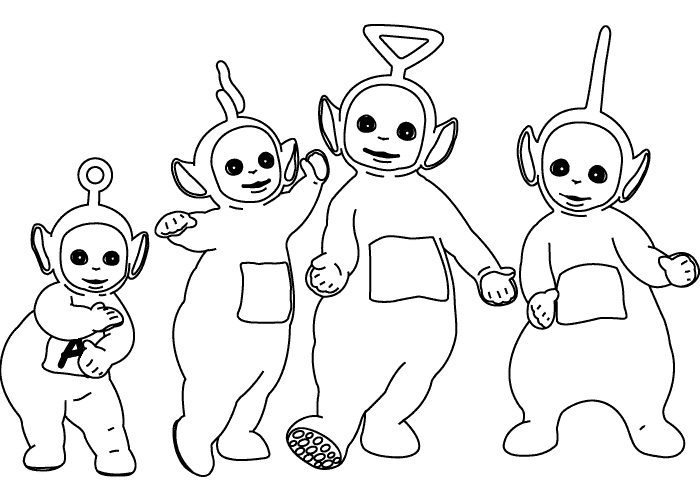
\includegraphics[width=1\textwidth]{a.png}
  \caption{正面照\upcite{dsd_tech2}}
  \label{fig:正面}
  \end{minipage}
  \begin{minipage}[b]{0.4\textwidth} %minipage宽
  \centering
  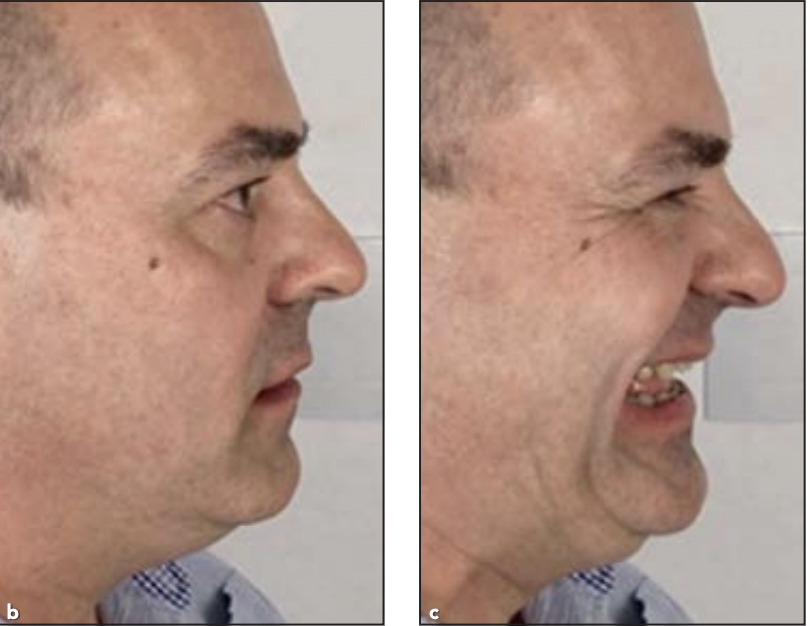
\includegraphics[width=1\textwidth]{paste_src/2023-02-07-20-50-39.png}
  \caption{側面照\upcite{dsd_tech2}}
  \label{fig:側面}
  \end{minipage}
  \end{figure}
  
\begin{figure}[H]%與文字並排
    \centering %圖片全居中
    %並排幾個圖就要開幾個minipage
    \begin{minipage}[b]{0.4\textwidth} %minipage寬
      \centering %图片局部居中
      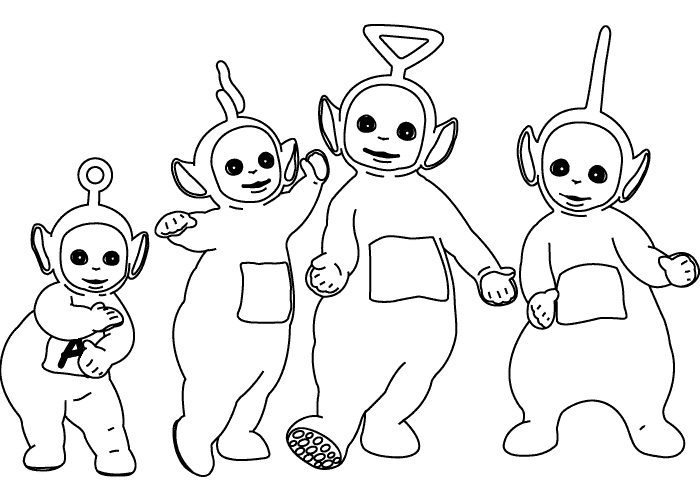
\includegraphics[width=0.8\textwidth]{a.png}
      \caption{最右邊是迪西}
      \label{fig:迪西}
    \end{minipage}
    \begin{minipage}[b]{0.4\textwidth} %minipage宽
      \centering %图片局部居中
      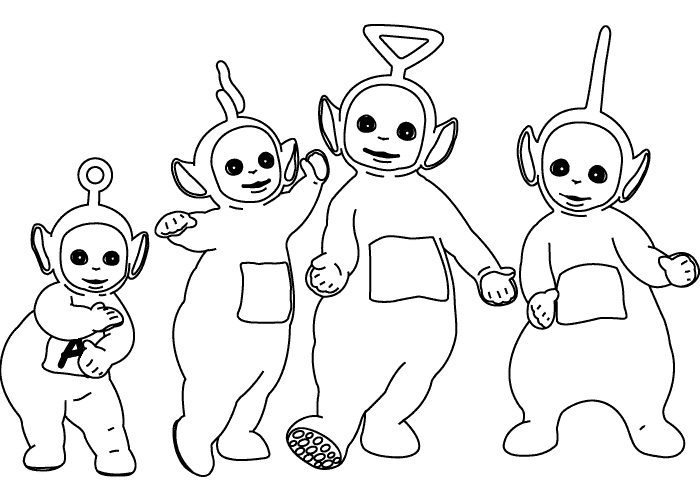
\includegraphics[width=0.8\textwidth]{a.png}
      \caption{再來是丁丁}
      \label{fig:丁丁}
    \end{minipage}
  \end{figure}
  所以
  丁丁是\prettyref{fig:丁丁}
  迪西是\prettyref{fig:迪西}




\section{My Chemical LaTeX}
  \subsection*{一些語法}
  
  \ce{2[AgCl2]-}\\
  \begin{minipage}[b]{0.3\textwidth}
    \centering
    \chemfig{*6(-=-=-=)}\\
    \chemfig{*5(-----)}\\
  \end{minipage}\\
  
  \chemfig{*6(-=-=-=)}\\
  \chemfig{*5(-----)}\\
  \chemfig{A-B}\\
  \chemfig{A=B}\\
  \chemfig{A~B}\\
  \chemfig{A>B}\\
  \chemfig{A>:B}\\
  \chemfig{A>|B}\\
  \chemfig{C(-[1]1)(-[2]2)(-[3]3)(-[4]4)(-[5]5)(-[6]6)(-[7]7)(-[0]0)}
  \ex 乙烯
  \chemfig{C(-[3]H)(-[5]H)=C(-[1]H)(-[7]H)}
  aaa

  


    

































\section{讀流程圖}

\begin{figure}[!htp]
  \centering
  \begin{tikzpicture}[node distance=2cm]

  \node (start) [startstop] {用戶透過手機app或是網頁拍攝微笑照片};
  \node (input1) [process,below of=start] {照片上傳伺服器};
  \node (process1) [process,below of=input1] {伺服器即時自動分析微笑照片};
  \node (out) [startstop,below of=process1] {將分析結果回傳到手機};


  \draw [arrow] (start) -- (input1);
  \draw [arrow] (input1) -- (process1);
  \draw [arrow] (process1) -- (out);


  \end{tikzpicture}
\end{figure}


\newpage
\tikz[remember picture,overlay] \node[opacity=0.3,inner sep=0pt] at (current page.center){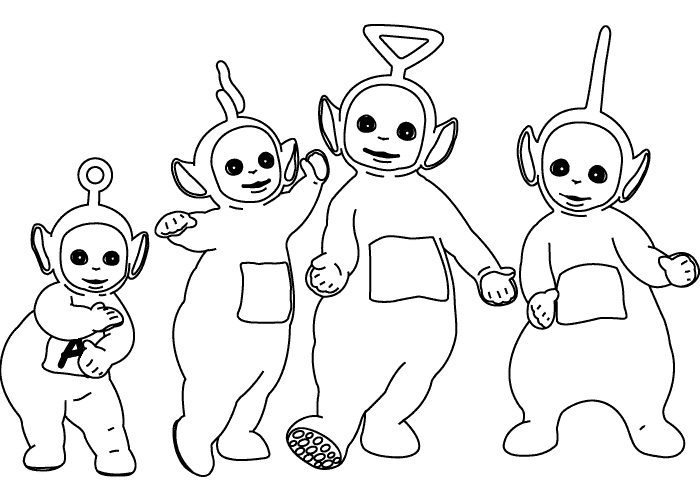
\includegraphics[width=\paperwidth,height=\paperheight]{a.png}};
\section{背景}
\subsection{tikz 實現}
編譯第一次會怪怪的,再一次就ok
\clearpage


\newpage



\AddToShipoutPictureBG*{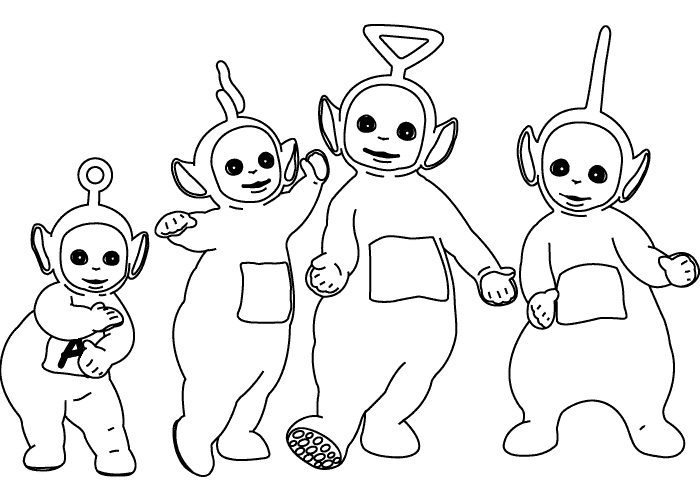
\includegraphics[width=\paperwidth,height=\paperheight]{a.png}}

\subsection{eso-pic}
text
\clearpage

\section{怪東西}


\bibliography{bibfile} 
\bibliographystyle{unsrt}


\end{document}
